\section{Мгновенный центр вращения}

%1
\AddProb Колесо радиуса $R$ катится без проскальзывания по горизонтальной поверхности со скоростью $v$. 
Найдите скорости различных точек колеса, уравнения траектории и радиус кривизны траектории в верхней точке дуги для произвольной точки на ободе колеса.

\AddProb Скорость одного конца стержня равна $v$ и направлена под углом $\alpha$ к стержню. 
Найдите скорость другого конца, которая направлена под углом $\beta$ к стержню.

\AddProb По гладкому горизонтальному столу свободно скользит тонкая прямая однородная палочка длины $L$. 
В некоторый момент скорость одного из концов равна $v$ и составляет прямой угол с палочкой, 
а скорость другого конца по величине равна $2v$. За какое время палочка повернется на угол $2\pi$?

\begin{wrapfigure}{r}{4.5cm}
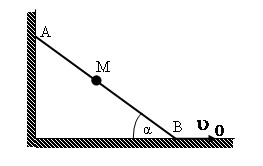
\includegraphics[width=4.5cm]{032006RotationKinematicsBar.jpg}
\end{wrapfigure}

\AddProb (2006) Между двумя стенками, образующими прямой угол, движется по направляющим без отрыва стержень АВ длиной $l_0$. 
Скорость точки В постоянна, равна $v_0$ и направлена горизонтально. Определить скорость $v$ и ускорение $a$  точки М, 
расположенной на расстоянии MB = $l$ от точки В, в момент времени, когда угол между горизонтальной стенкой и стержнем АВ составляет $\alpha$.


\section{Бесконечно малые перемещения}

%6
\AddProb Тело движется по окружности радиуса $R$ так, что его скорость зависит от времени по линейному закону: $v = at$. 
Найдите зависимость ускорения тела от времени.

\begin{wrapfigure}{r}{3.0cm}
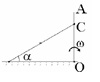
\includegraphics{0307InfinitesimalChangeRay.jpg}
\end{wrapfigure}

\AddProb Луч света падает на вращающийся экран AO, образуя на нем зайчик C. Угловая скорость вращения экрана $\omega$\,; 
угол, образуемый лучом света с горизонтом, равен $\alpha$. В некоторый момент времени экран занимает положение, 
изображенное на рисунке, при этом расстояние от оси вращения до зайчика OC = $l$. 
Определите, какую скорость имеет зайчик относительно экрана в указанный момент времени.

\begin{wrapfigure}{r}{3.0cm}
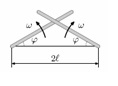
\includegraphics{0308RotationKinematicsProjectors.jpg}
\end{wrapfigure}

\AddProb Определить скорость точки пересечения двух лучей прожекторов, 
которые вращаются в противоположных направлениях с угловой скоростью $\omega$, в момент, 
когда угол наклона к горизонту обоих прожекторов равен $\varphi$. Расстояние между прожекторами равно $2l$.

\begin{wrapfigure}{r}{3.0cm}
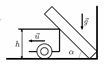
\includegraphics{0309RotationKinematicsLorry.jpg}
\end{wrapfigure}

\AddProb Бревно, упираясь одним концом в угол между землей и стеной, касается грузовика на высоте $h$, 
который отъезжает от стены со скоростью $u$. Как зависит угловая скорость вращения бревна от угла $\alpha$ между бревном и горизонтом?

\AddProb За лисой, бегущей прямолинейно с постоянной скоростью $v$, бежит собака таким образом, 
что ее скорость $u$ всегда направлена на местоположение лисы. В момент, когда векторы скоростей перпендикулярны, 
расстояние между ними было равно $L$. С каким ускорением при этом двигалась собака?

\begin{wrapfigure}{r}{3.0cm}
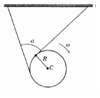
\includegraphics{0311RotationKinematicsDisc.jpg}
\end{wrapfigure}

%11
\AddProb На диск радиуса R намотаны две нерастяжимые нити, закрепленные в двух разных точках. 
При отпускании диск вращается. Когда угол между нитями у диска $\alpha$, угловая скорость вращения диска $\omega$. 
С какой скоростью в этот момент движется центр диска? Нити остаются натянутыми.

\AddProb Внутри неподвижной окружности катится без скольжения другая окружность вдвое меньшего радиуса. 
Какую траекторию описывает при этом произвольно выбранная точка на подвижной окружности?

\begin{wrapfigure}{r}{2cm}
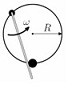
\includegraphics{0313RotationKinematicsRingAndBead.jpg}
\end{wrapfigure}

\AddProb Бусинка может двигаться по кольцу радиуса $R$, подталкиваемая спицей, 
которая вращается с угловой скоростью $\omega$ в плоскости кольца. Ось вращения спицы находится на кольце. Определить ускорение бусинки.

\AddProb По палочке, которая вращается с угловой скоростью $\omega$, ползет жук со скоростью $v$. 
Определите скорость и ускорение жука, когда он находится на расстоянии $L$ от оси вращения палочки.

\AddProb (2003) Четыре черепахи находятся в вершинах квадрата со стороной $l$. Они начинают двигаться одновременно с постоянной скоростью $v$. 
Каждая черепаха движется по направлению к своей соседке по часовой стрелке. Где встретятся черепахи и через какое время? 
Найти угол между скоростью движения черепахи и одной из сторон квадрата как функцию ее координат $\varphi = \varphi (x,y)$.
